\documentclass[master.tex]{subfiles}
 
\begin{document}


In this chapter the used optimization methods are described and evaluated. Since a deeper discussion would be out of scope only a brief overview is given. Currently almost 50\% of the simulation time is spend on the SOR-Solver for the polarization equation. As a consequence most of the work was spend on the SOR-Solver.
\section{OpenMP}
The complete calculation of the \ac{rhs} for the density and parallel velocities equations can be parallelized without negative consequences. Most gain gives us the parallelization over the z-direction. This is achieved with a simple OpenMP \textit{"taskloop"} worksharing construct as is it is described in \autoref{sec:open-mp-method}. Parallelization in x-direction is only effective for 2D simulations or for very high resolutions. Using the construct on the y-direction is not useful since this loop is always vectorized by the compiler yielding much higher performance. Since the SOR-Solver only works in xy-direction the parallelization in z-direction is effective as well (each solver XY-Plane is solved in parallel). Furthermore sections parallelism is implemented where possible.

\section{Nvidia-CUDA}
To further optimize the SOR-solver and reduce execution time the iteration is moved to the graphics card. This creates some overhead since data has to be moved back and forth to the GPU. Also since there is usually only one GPU available the parallelization in z-direction is not possible anymore. Scaling for different systems is presented later. The kernel implementation uses the speedup gained from \textit{Shared Memory} access in connection to coalesced memory loading.

\section{Evaluation}
To evaluate performance in a realistic situation it is measured using an actual simulation. A single measurement consists of 1000 iterations where the execution time is measured each 20 iterations. Also measured is how much the different steps of each iteration take.\newline
The code is evaluated on three different systems:
\begin{itemize}
    \item \textbf{\ac{K40}}: Intel Xeon E3-1225 V2; 16GB RAM; Nvidia K40
    \item \textbf{\ac{GTX}}: 2x Intel Xeon Bronze 3104; 12x 8GB RAM; 7x Nvidia GTX 1080 Ti
    \item \textbf{\ac{TV}}: 2x Intel Xeon Gold 6130; 12x 16GB RAM; 4x Nvidia Titan V
\end{itemize}
Two versions are tested against each other. The first version only runs on the CPU. The second version executes the \ac{SOR}-Solver and the Fourier transformation associated with gyroaveraging on the GPU(s). Both versions are compiled with \textit{-march=native -O3} and for the different systems the corresponding cuda compute architecture versions. Four different resolutions (z,x,y) are tested:
\begin{enumerate}
    \item 8x128x128
    \item 8x128x256
    \item 8x256x512
    \item 8x512x1024
\end{enumerate}

\subsection{Data Output}
Five sections of the code are measured individually as well as the global execution time:
\begin{itemize}
    \item Polarization Equation
    \item Gyroaveraging
    \item Right Hand Side (RHS) of Equations (\textit{calculation of $F(\Phi)^{n+1}$ in \autoref{eq:karnidakis-scheme}})
    \item Time Stepping (\textit{Calculation of \autoref{eq:karnidakis-scheme}})
    \item External Boundaries (involves gyroaveraging)
\end{itemize}
Each data point taken is the mean value out of 20 iterations. In \autoref{fig:k40_gpu_vs_cpu} the complete data set for 8x128x128 on the \ac{K40} and \ac{K40C} systems is presented. It is clearly visible that the first point represents an outlier which is explained by the fact that the initial value for the polarization solver is far off from the solution. It is therefore excluded from further evaluations. 

\begin{figure}[!hbtp]
    \centering
    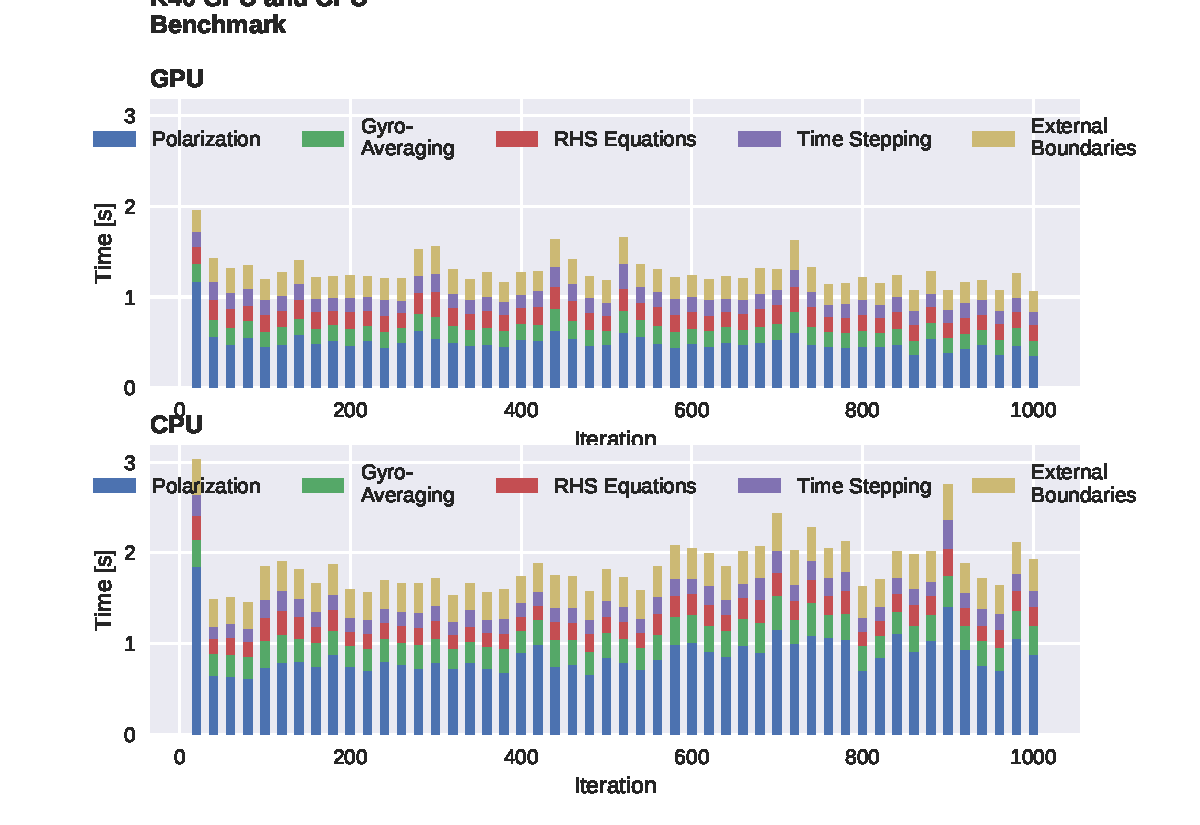
\includegraphics[width=\linewidth]{pdfs/k40CPUvsGPU_full.pdf}
    \caption{\small Example of performance run. Timings are taken every 20 iterations. Comparison for 8x128x128 on K40 workstation}
    \label{fig:k40_gpu_vs_cpu}
\end{figure}

\autoref{fig:k40_gpu_vs_cpu_mean} shows the mean duration of each step. There is no significant difference visible in "Time Stepping" and "RHS Equations". This is expected since both steps are fully executed on the CPU. One can however already see a performance improvement for the other steps. \autoref{tab:talbe_k40_k40c} presents the quantitative results. The GPU scales better with grid size even though this is a perfectly parallelizeable problem for the CPU where each core calculates one xy-layer in z-direction. Speedups >2 are observed.
The larger errors associated with the CPU version especially for the polarization may be explained by the scheduler of the operation system. More information on scheduling on linux systems and the negative impact can be found here \cite{Scheduling-Linux}.

\begin{figure}[!hbtp]
    \centering
    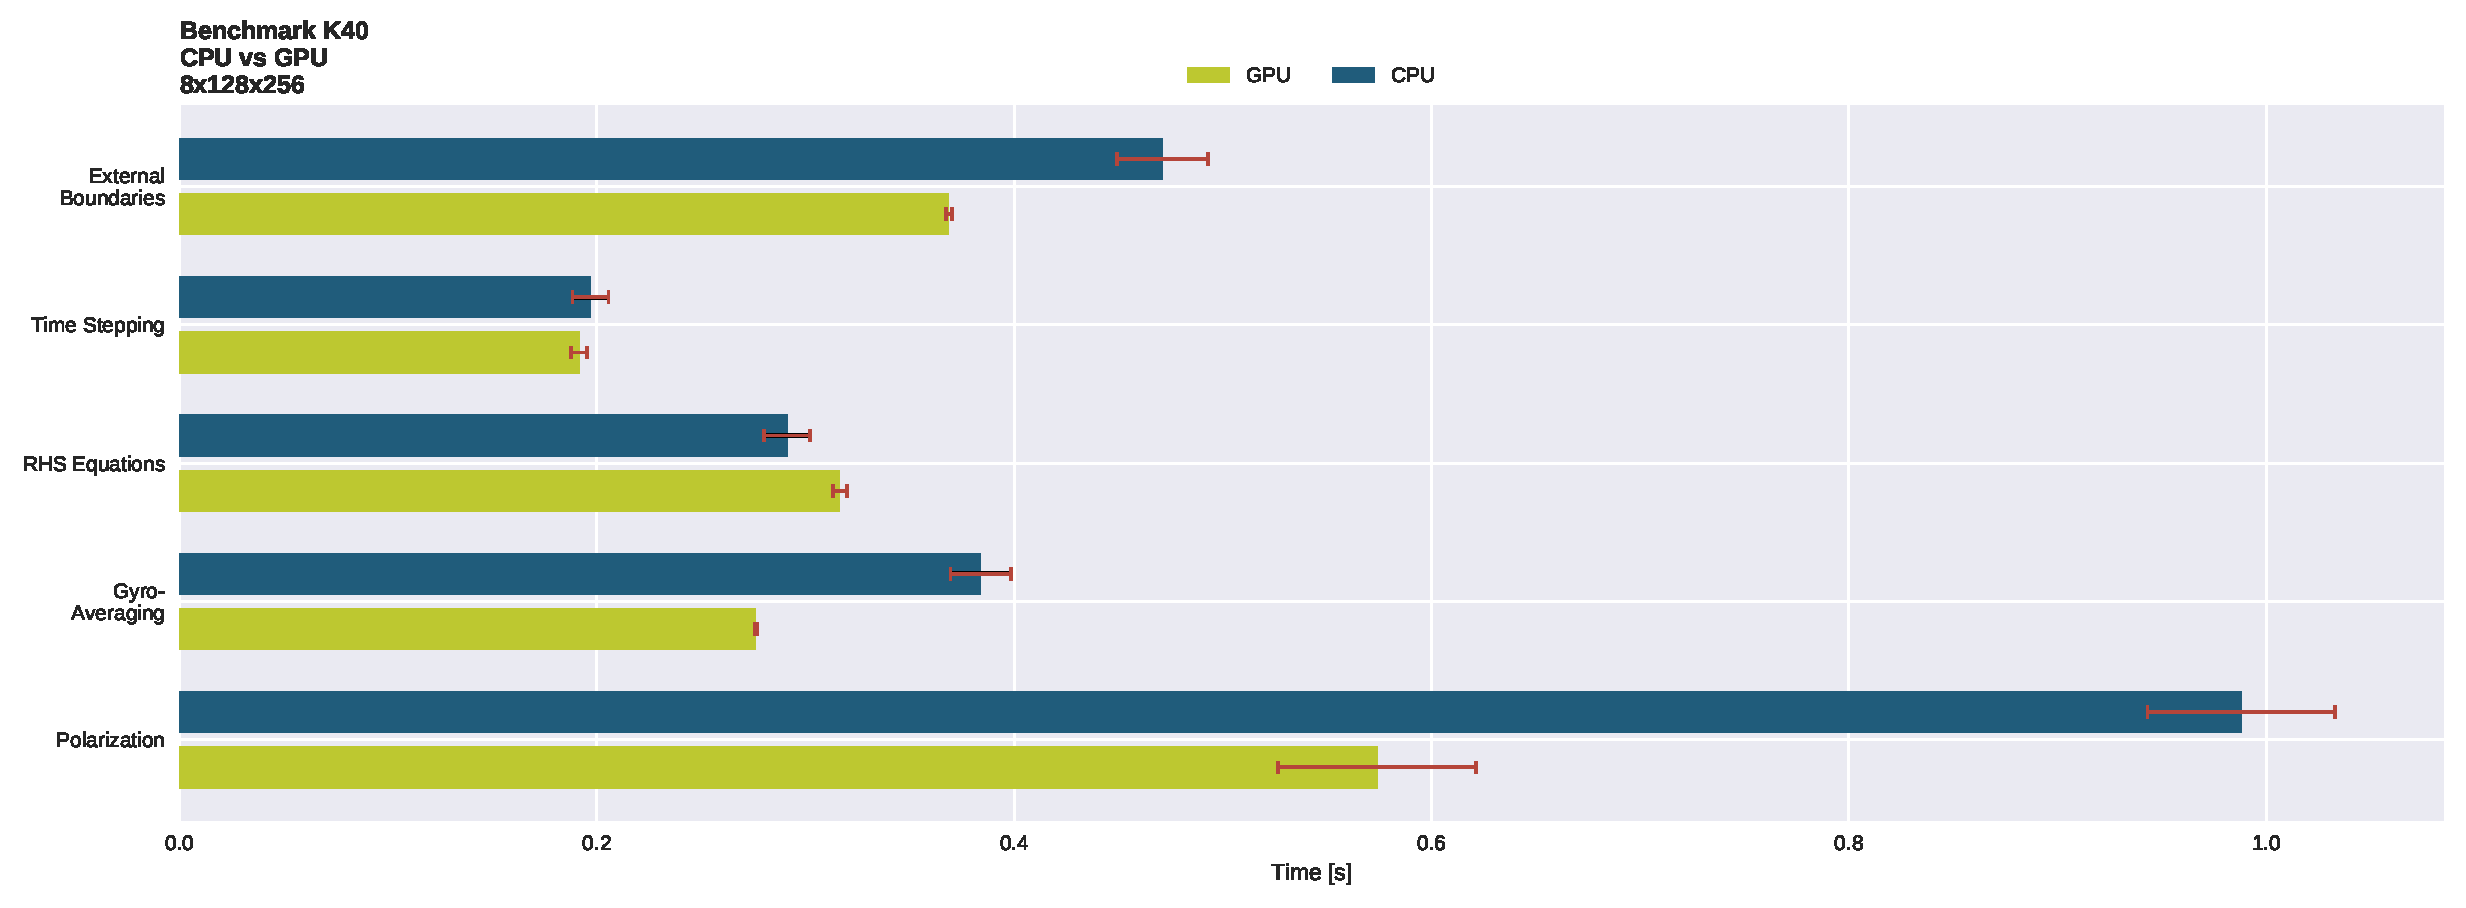
\includegraphics[width=\linewidth]{pdfs/k40CPUvsGPU_means.pdf}
    \caption{\small Mean and standard deviation of timings measurement presented in \autoref{fig:k40_gpu_vs_cpu} omitting the first data point.}
    \label{fig:k40_gpu_vs_cpu_mean}
\end{figure}

\begin{figure}[!hbtp]
    \centering
    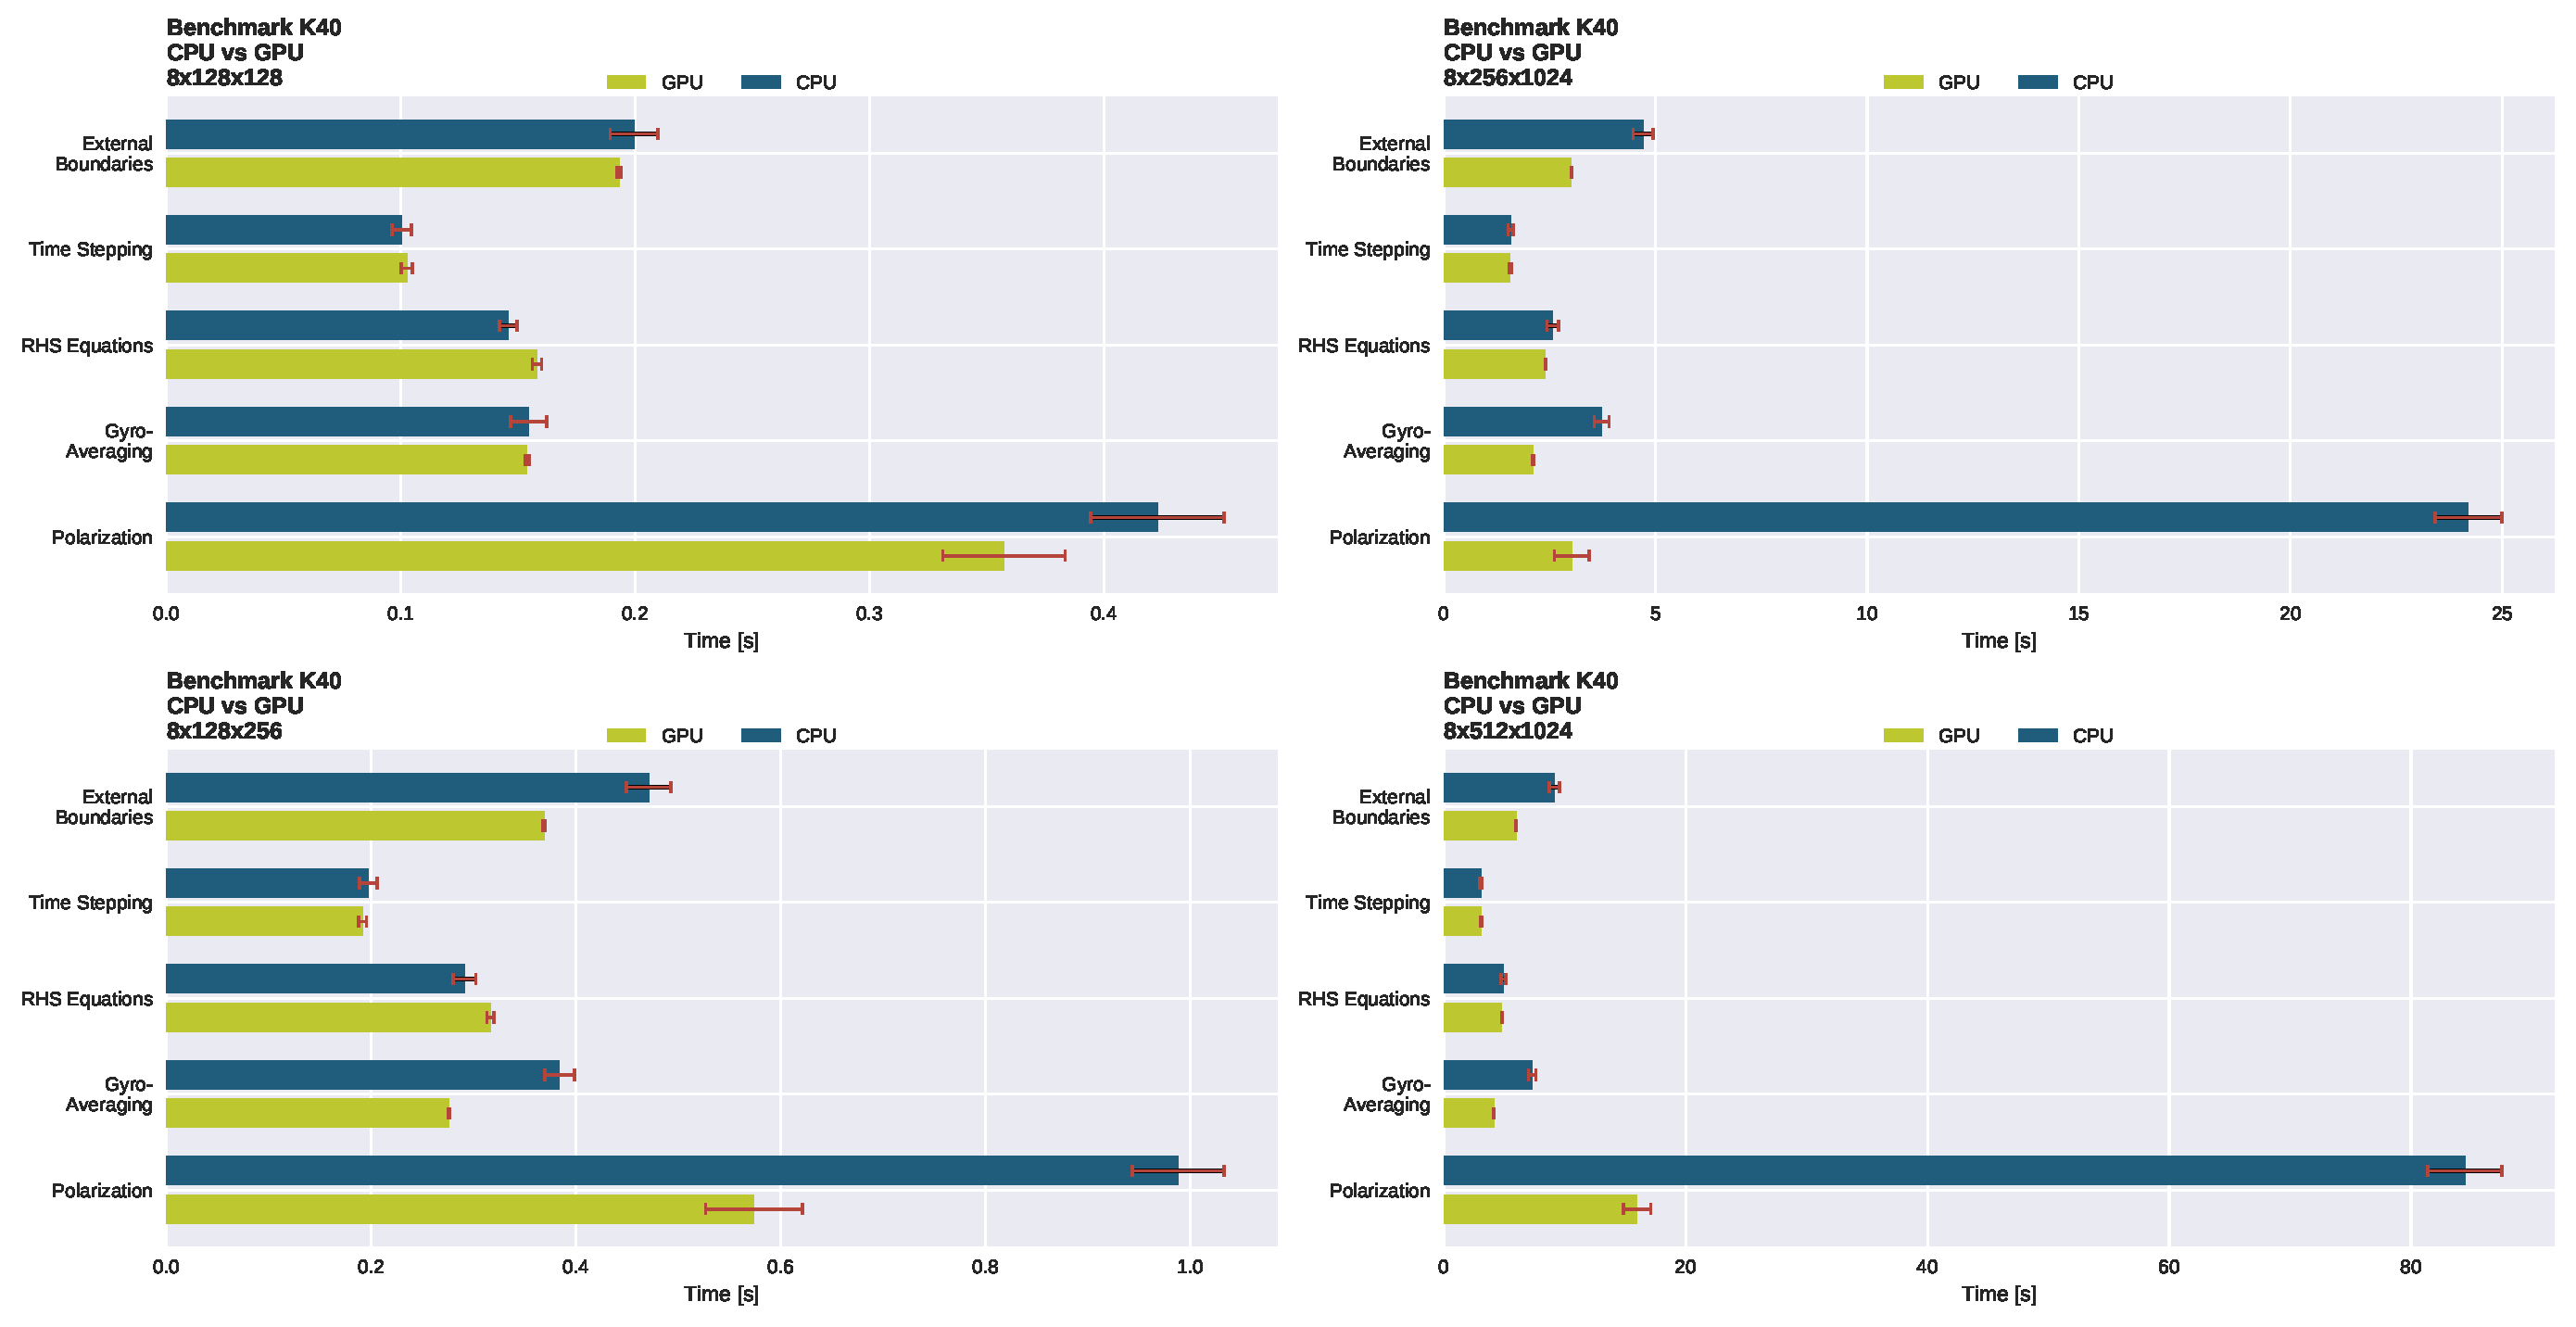
\includegraphics[width=\linewidth]{pdfs/k40CPUvsGPU_complete_means.pdf}
    \caption{\small Comparison of \ac{K40} and \ac{K40C} for all resolutions.}
    \label{fig:k40_gpu_vs_cpu_complete_means}
\end{figure}

\begin{table}[!hbtp]
    \centering
    \begin{tabular}{c|c|c|c}
        Grid Size & \ac{K40} & \ac{K40C} & GPU Speedup  \\  \hline
        8x128x128 & $1.89 \pm 0.28$s & $1.32 \pm 0.15$s & $1.43 \pm  0.27$ \\
        8x128x256 & $3.76\pm0.42$s & $2.38\pm0.19$s & $1.58\pm0.21$ \\
        8x256x512 & $17.92\pm4.13$s & $8.10\pm0.40$s & $2.21\pm0.52$ \\
        8x256x1024 & $36.27\pm8.19$s & $16.85\pm0.76$s & $2.15\pm0.50$ \\
        8x512x1024 & $70.05\pm25.02$s & $40.45\pm2.84$s & $1.73\pm0.63$
    \end{tabular}
    \caption{Execution times of 20 iterations for \ac{K40} and \ac{K40C} and speedup of GPU version against CPU version}
    \label{tab:talbe_k40_k40c}
\end{table}
\newpage
\subsection{Results for Multi GPU Systems}
Further on results for multi GPU systems are presented. For each system the execution time using only the CPU is compared to the execution time where all available GPU devices are used as well. The results for mean execution time of 20 iterations (again omitting the first 20) are plotted in \autoref{fig:all_systems_resolution_scaling}. Generally the CPU version scales worse than the GPU version. The GTX node almost reaches a speedup of three compared to the CPU version. Considering the execution time of almost ~3s per iteration, running a simulation with 200.000 iterations takes 
almost seven days using the CPU version whereas it only takes two and a half days using the GPU version. 
\begin{figure}[!hbtp]
    \centering
    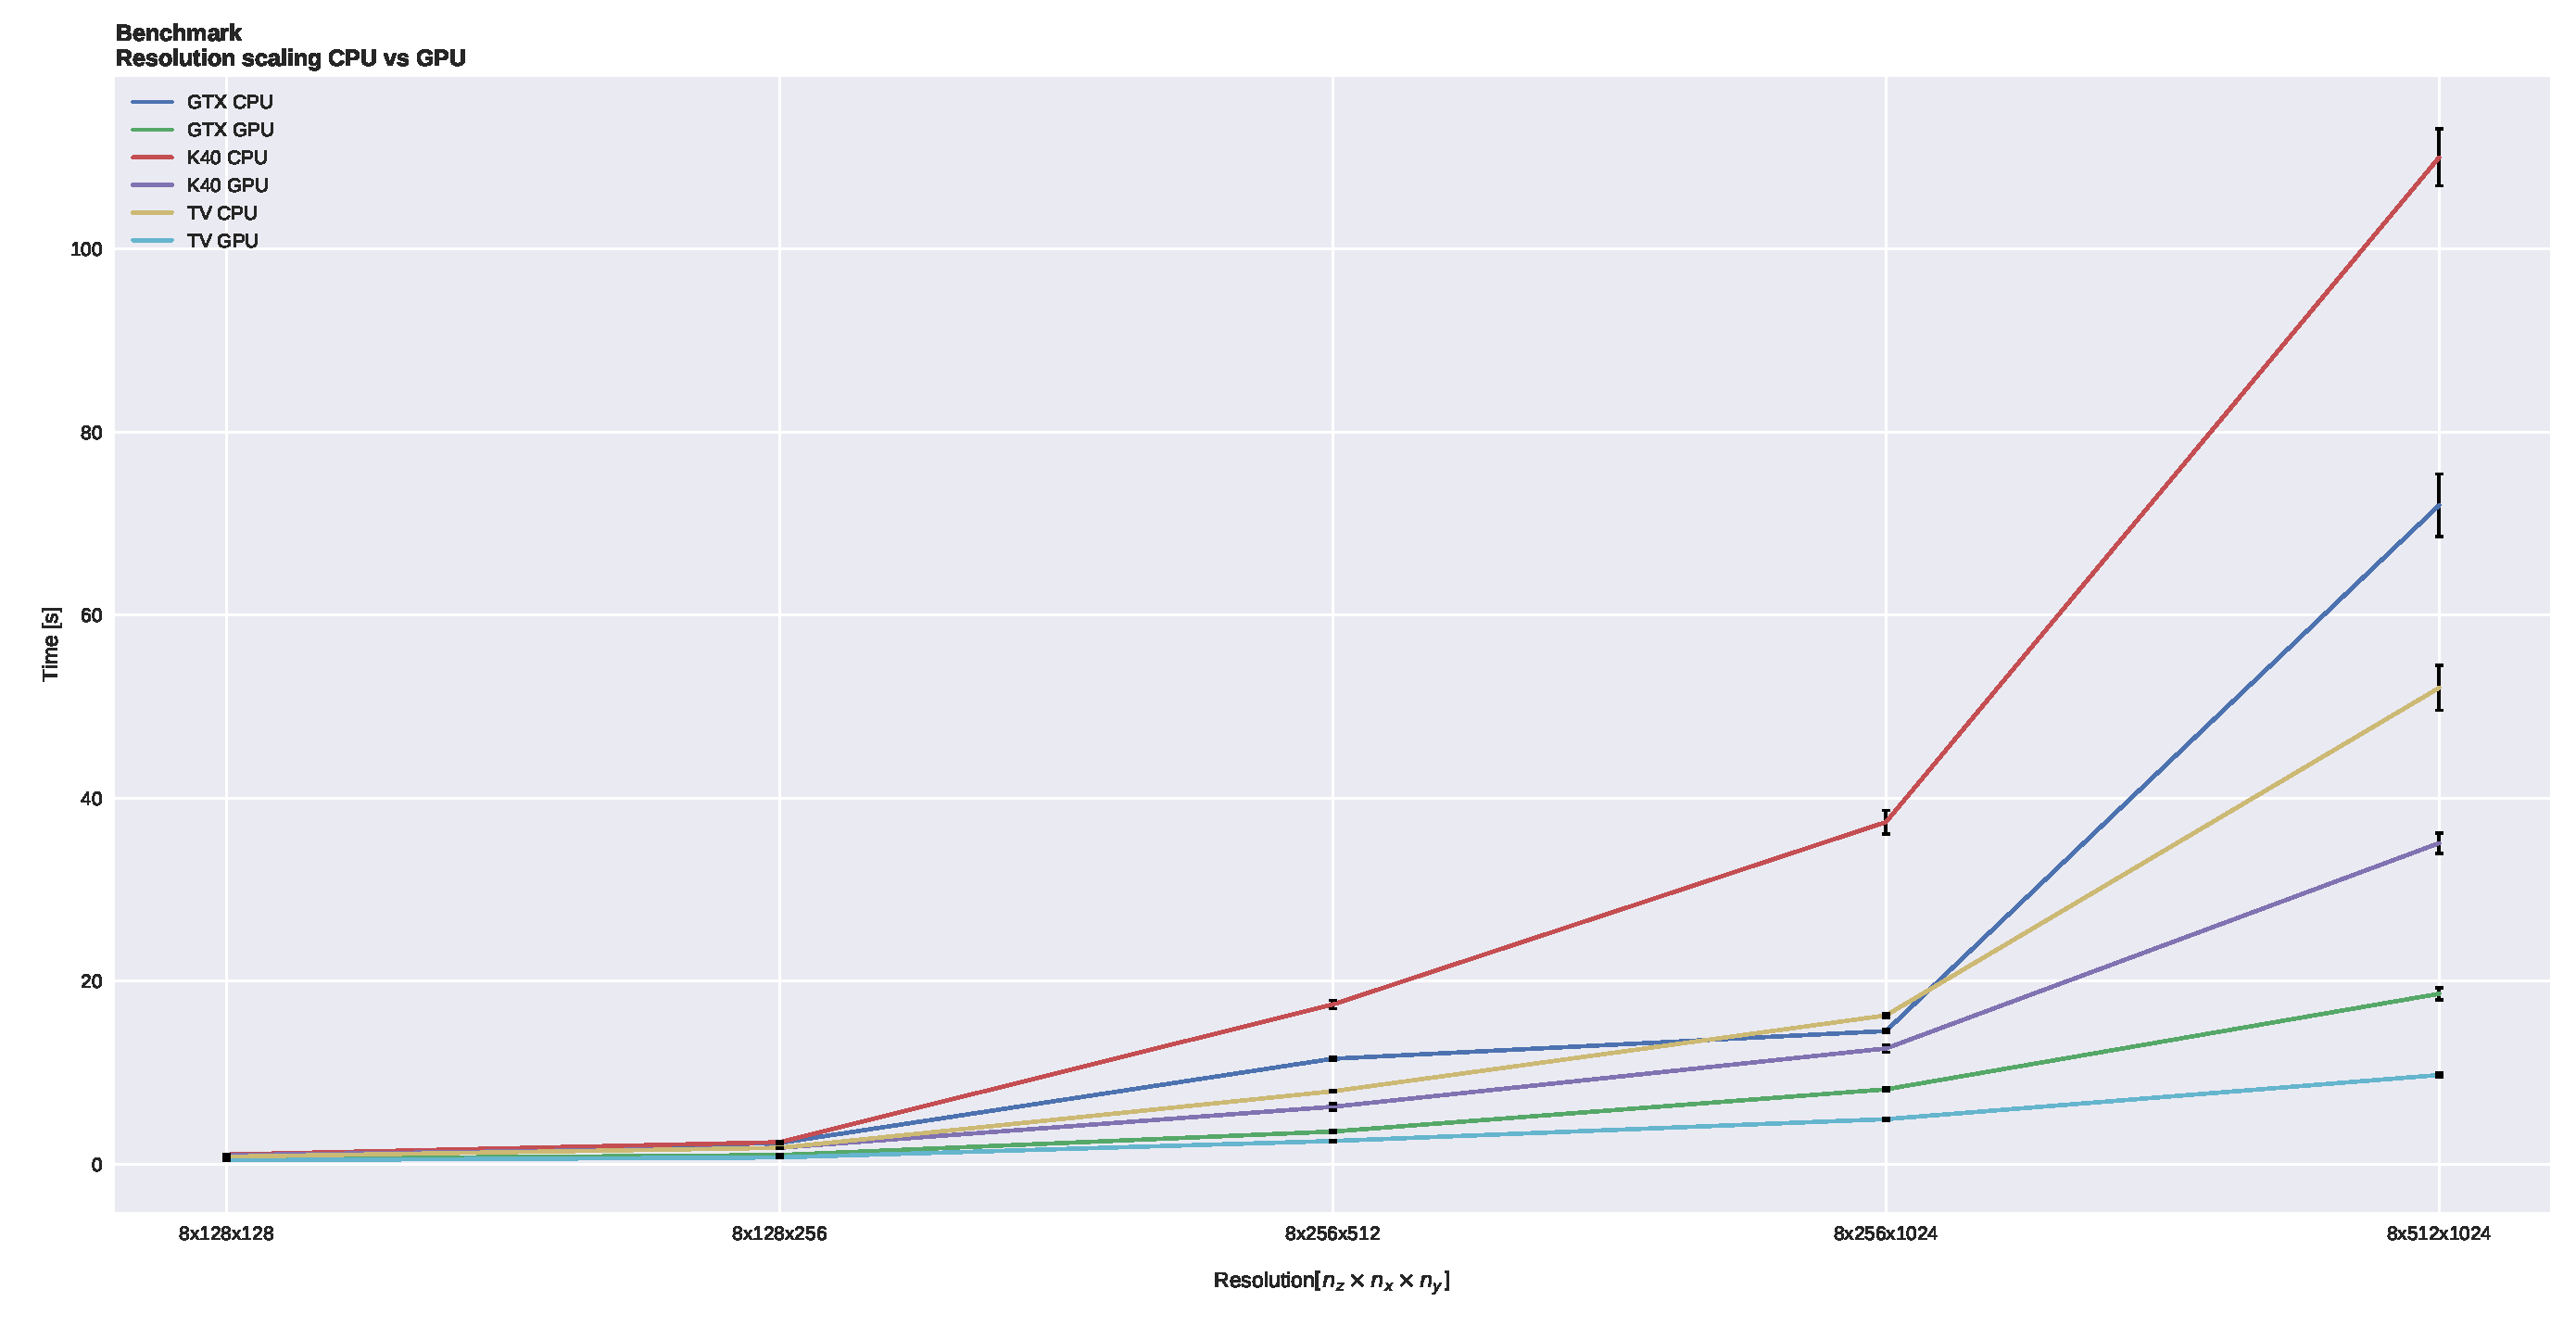
\includegraphics[width=\linewidth]{pdfs/all_systems_compared.pdf}
    \caption{\small Resolution scaling on all three systems. The GPU version genrally scales better.}
    \label{fig:all_systems_resolution_scaling}
\end{figure}

\subsection{Future Optimizations}
Using this data one can now determine where it is useful to do future optimizations. If we look at the normalized data from the \ac{GTX} system for a resolution of 8x256x1024 one can see that the most expensive part now became the time stepping (\autoref{fig:gtx_parts}).
\begin{figure}[!hbtp]
    \centering
    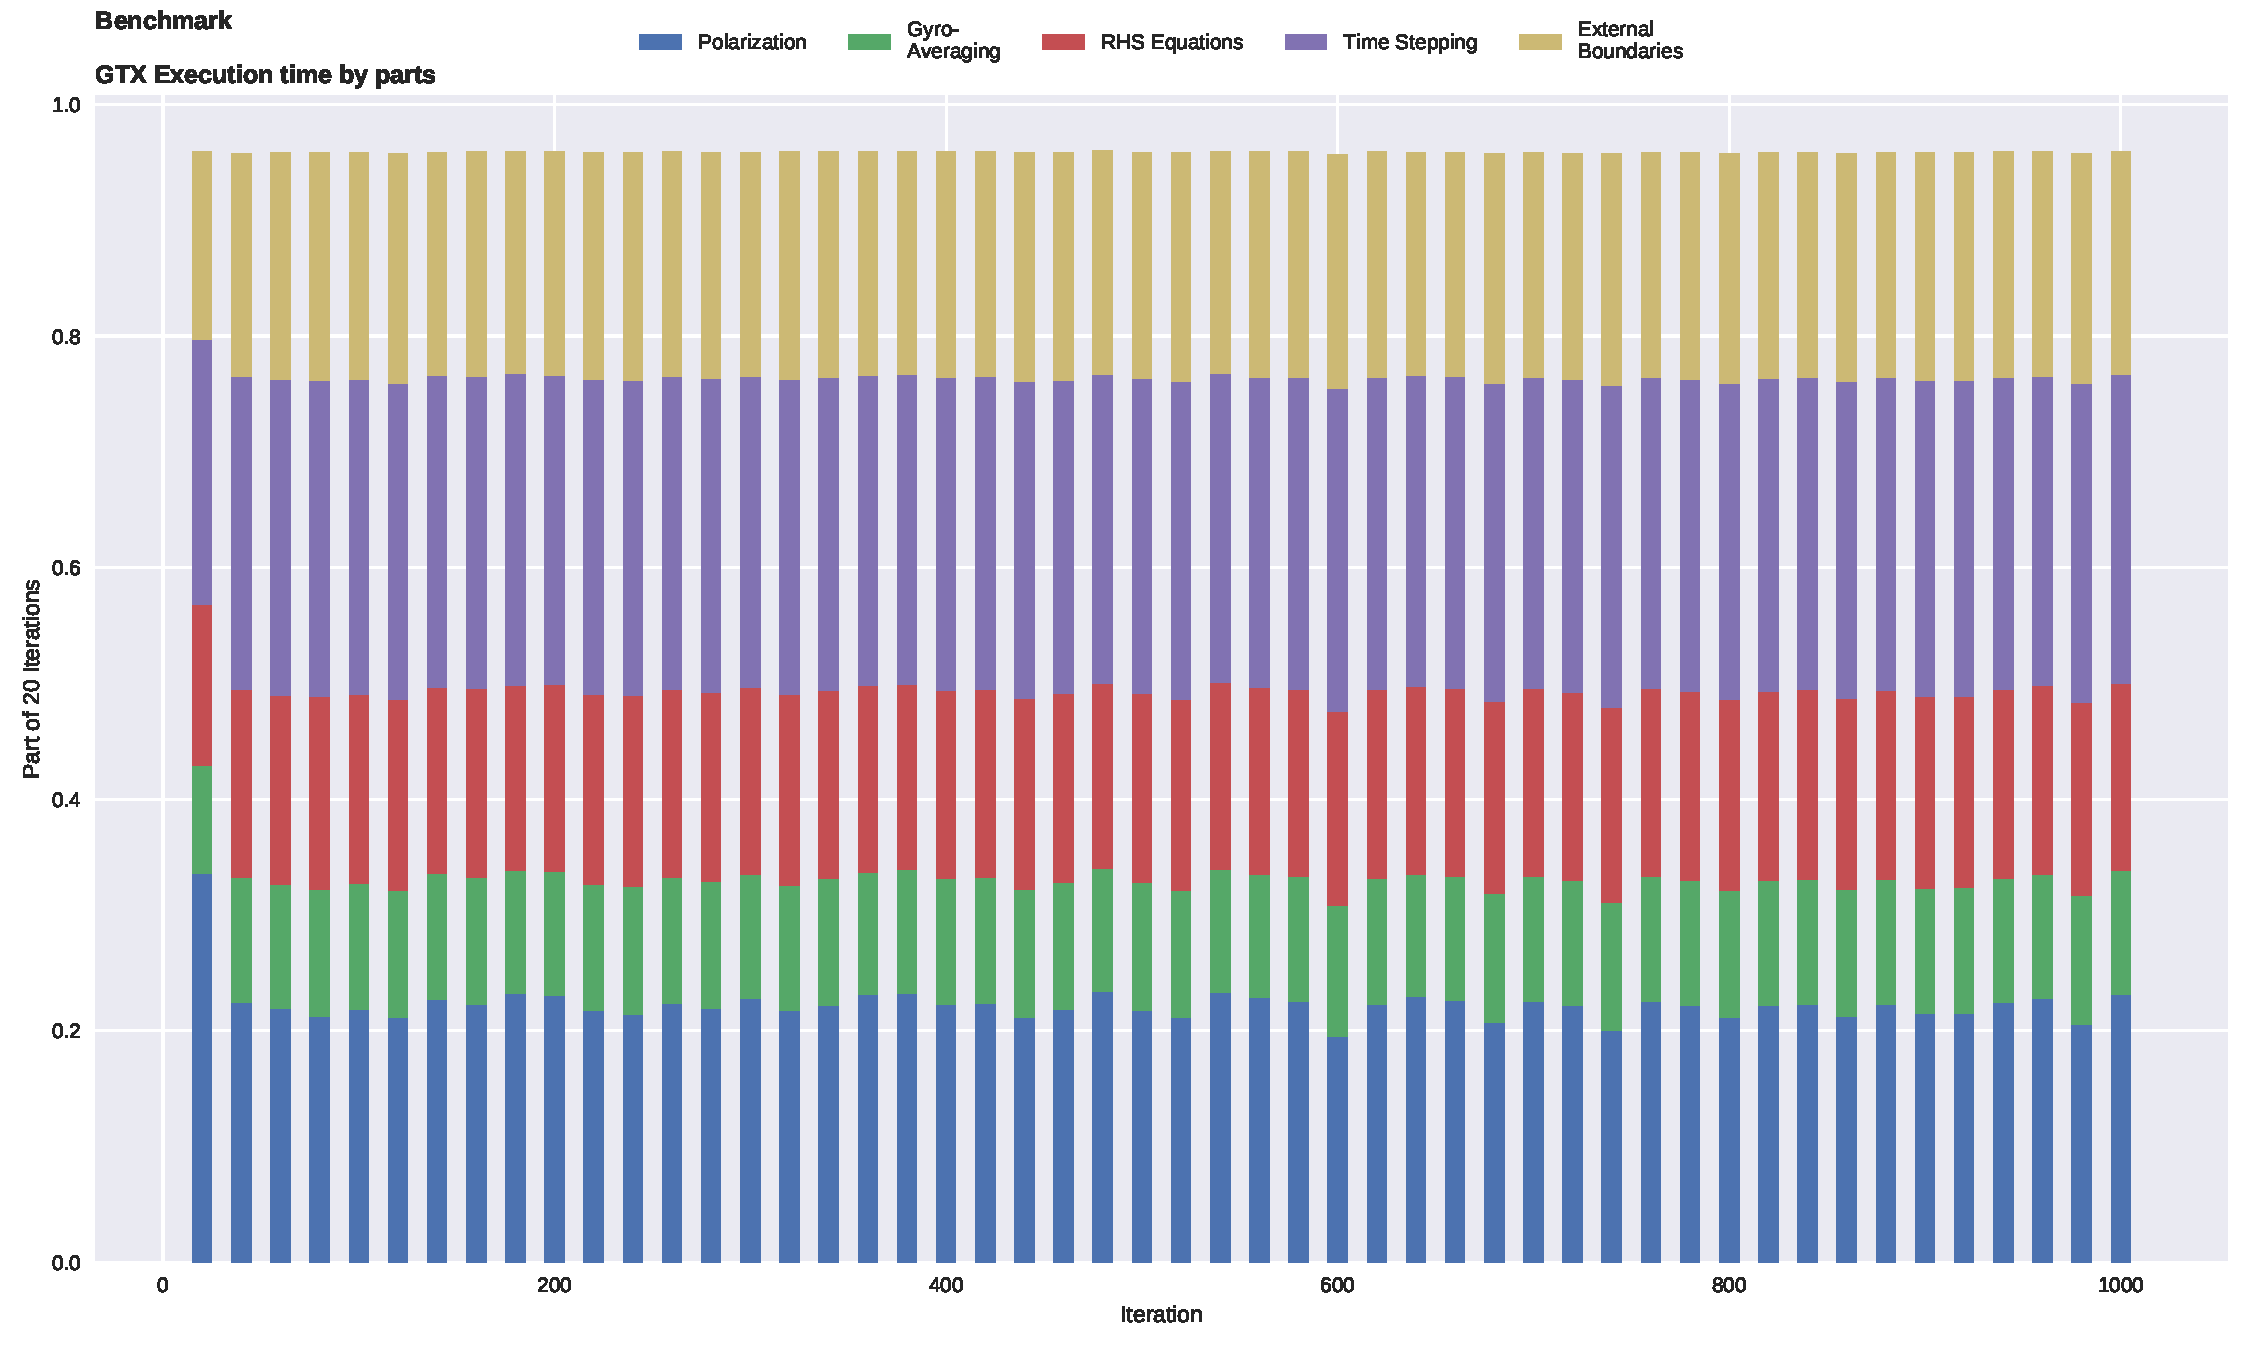
\includegraphics[width=\linewidth]{pdfs/gtx_parts.pdf}
    \caption{\small Execution times of 20 iterations normalized to the full execution time of these 20 iteartions.}
    \label{fig:gtx_parts}
\end{figure}
Moving the timestepping to the GPU as well as the \ac{RHS} evaluation would effectively fully move the simulation to GPU execution. Since less data transfers between host memory and device memory would be required this might dramatically increase performance, but data transfers between individual GPU's would be necessary to model the z-direction further increasing code complexity.

\section{Conclusion}
Speedups larger than two have been measured which at least reduces the execution time by a factor of two. The speedup is generally better the greater the grid is. This makes it possible to asses whether resolution has an impact on the simulation model. Prior to these optimization's running a simulation with grid size 8x256x1024 could take a week but is now possible in a few days allowing for faster prototyping of adjustments to the model. It should be noted though that magical speedups as they are described in \cite{CUDARedBlack} of >40 are not reached. A major positive effect on CPU performance has vectorization. Most of the simulation code is vectorized by the compiler and as such it runs very well on the CPU. Also the simulation does not have a high memory footprint since a single XY-plane takes about 25MB for a single quantity on a grid of 8x256x1024. Such a plane almost fits into the cache of current CPUs and naturally gives them a high memory bandwidth. Nevertheless it might be worth moving all the code to the GPU which would reduce the overhead associated with copying data from the host memory to the GPU memory. On the other hand this involves much more complex programming and in most cases exceeds the qualifications of a physicist thus making it harder to collaborate or evolve the model and simulation.



\end{document}